\scanpage{4}
\mspage{3}
\uline{\unsure{Remarque|Remarques}} \deleted{Si \unsure{de|dans} \unsure{\textcircled{1}} $2^\circ)$,} \inserted{$1^\circ)$} La condition $\beta)$ de $2^\circ$ est automatique si $\unsure{\mathscr{L}|\mathcal{L}}$ fini, plus gén. si $\mathscr{L}$ est ``artinien'' pour $\subset$, i.e. s'il n'existe pas de suite str. décroissante d'éléments de $\mathscr{L}$
\[
 A_1\supset A_2\supset\ldots
\]
Si par contre $\mathscr{L}$ est réduit à \deleted{\unsure{une telle}} \inserted{\unsure{l'ens des}} termes d'une telle suite, \deleted{\unsure{alors} \illegible{1}} alors $\alpha$ est satisfaite mais non $\beta$ si $\displaystyle\bigcap A_i\ne\varnothing$.

$2^\circ)$ Dans $3^\circ$, \deleted{il suffit de supposer} la condition $\eta)$ n'est pas surabondante,
\[
\left\{\begin{aligned}
 &\deleted{\displaystyle\bigcup_{A\in\mathscr{L}'}A^\circ=|\mathscr{L}|}\\
 &\deleted{\displaystyle\forall A\in\mathscr{L},\ \text{on a } A=\bigcup_{\substack{B\in\mathscr{L}\\\text{t.q. }B^\circ\subset A}}B^\circ}
\end{aligned}\right.
\]
comme on voit dans l'exemple suivant
\[
\deleted{\mathscr{L}=\{A,B,C,D\}\quad\text{\deleted{\unsure{de}} \unsure{sur|où}}\ L=\{x,y,z,t\}}
\]
\figure{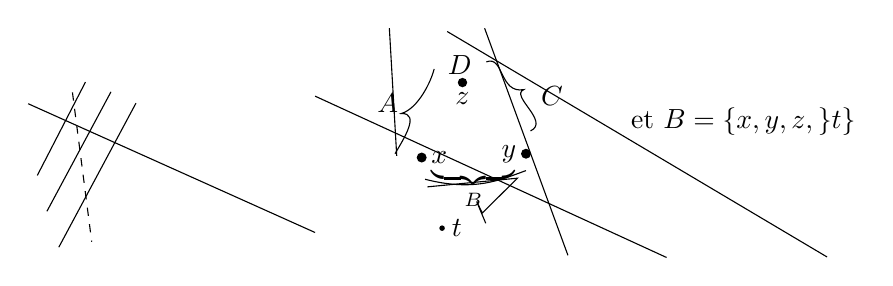
\begin{tikzpicture}[x=0.72cm,y=0.69cm,baseline]
\node at (2.05,2.18) {$\deleted{D}$};
\fill (2.10,1.85) circle (1.7pt) node[below] {$\deleted{z}$};
\fill (1.38,0.47) circle (1.8pt) node[right] {$\deleted{x}$};
\fill (3.22,0.54) circle (1.8pt) node[left] {$\deleted{y}$};
\fill (1.74,-0.83) circle (1pt) node[right] {$\deleted{t}$};
\node at (0.78,1.47) {$\deleted{A}$}; \node at (3.68,1.60) {$\deleted{C}$};
\draw (1.60,2.10) .. controls (1.55,1.88) and (1.32,1.37) .. (1.02,1.28)
 .. controls (1.36,1.29) and (1.06,.81) .. (.91,.54);
\draw (2.52,2.23) .. controls (2.83,2.36) and (2.75,1.64) .. (3.18,1.72)
 .. controls (2.93,1.61) and (3.65,1.13) .. (3.30,.96);
\node at (2.29,-.10) {$\deleted{\unsure{\underbrace{\hspace{3em}}_{B}}}$};
\draw (1.44,.07) .. controls (2.30,-.16) and (2.75,.05) .. (3.22,.23);
\draw (1.48,-.07)--(3.07,.09)--(2.45,-.55)--(2.35,-.34)--(2.51,-.74);
\node[right] at (4.9,1.14) {\deleted{et $B=\{x,y,z,\deleted{\unsure{\}}}t\}$}};
\draw[thin] (-4.55,1.86)--(-5.40,.14) (-4.10,1.68)--(-5.23,-.52) (-3.66,1.47)--(-5.02,-1.18);
\draw[dashed,thin] (-4.78,1.67)--(-4.44,-1.08);
\draw[thin] (-5.56,1.46)--(-.5,-.91);
\draw[thin] (-.5,1.60)--(5.70,-1.37); \draw[thin] (1.83,2.79)--(8.53,-1.36);
\draw[thin] (.81,2.85)--(.94,.50); \draw[thin] (2.49,2.85)--(3.96,-1.33);
\end{tikzpicture}}
\[
\deleted{A^\circ=\{x\},\ C^\circ=\{y\},\ D^\circ=\{z\},\ B^\circ=
\deleted{\unsure{\varnothing|\{z\}}}\{t\}}
\]
% slanted
\margin{Exemple idiot -- mais voir contre\unsure{xemple|exemple} correct (avec I \uline{infini}) GF \uline{VIII}, p\unsure{ges|ages} 44,45.}
\[
\begin{aligned}
 &\deleted{\mathscr{L}=\{A,B,C,D\}\qquad\text{avec}}\\
 &\deleted{A\cap C=D,\quad\deleted{\unsure{D|A}\unsure{\subset|=}\,B}}
\end{aligned}
\]
\diagram{\begin{tikzcd}[ampersand replacement=\&,row sep=1.1em,column sep=1em]
 \& \deleted{D} \arrow[dl,no head,bend right=45,shorten <=2pt,shorten >=2pt] \arrow[dr,no head,bend right=48,shorten <=2pt,shorten >=2pt] \& \\
 \deleted{A} \& \& \deleted{C} \arrow[dl,no head,bend left=8] \\
 \& \deleted{\unsure{B}}\deleted{B} \&
\end{tikzcd}}
\deleted{donc}
\[
\begin{aligned}
 &\deleted{\deleted{A^\circ=A\setminus D,\ \unsure{t|1}}}\\
 &\deleted{D^\circ=D,\ A^\circ=A\setminus D,\ C^\circ=C\setminus D,\ B^\circ=B\setminus(A\cup C)}
\end{aligned}
\]
\deleted{\deleted{On a $A^\circ\subset B$} On a $A^\circ\subset B$ mais non pas $A\subset B$. Ici \deleted{$A^\circ$} tous les $X^\circ$ $(X\in\mathscr{L})$ sont non vides.}

\margin{\deleted{[\unsure{\ensuremath{\delta}|\ensuremath{\eta}} \unsure{et} si $A\in\mathscr{L}\Rightarrow A\ne\varnothing$ ??]}}
\uline{Définition} On dit que $\mathscr{L}$ est \uline{préadmissible}, si elle satisfait les conditions équivalentes $1^\circ,2^\circ,3^\circ$. \unsure{!} On dit qu'elle est \uline{admissible} si de plus
